\section{Leggi di De Morgan}

Le leggi di De Morgan, sono relative alla \textbf{logica booleana}\footnote{è il ramo dell'algebra in cui le variabili possono assumere solamente i valori vero e falso} e stabiliscono relazioni di equivalenza tra gli operatori di congiunzione e disgiunzione logica.
Le due leggi di De Morgan per unione ed intersezione (potremmo applicare le leggi anche ad altre operazioni) permettono di esprimere il complementare dell'intersezione e il complementare dell'unione in una forma alternativa:
\begin{align}
    \overline{A \cup B} &= \overline{A} \cap \overline{B} \\
    \overline{A \cap B} &= \overline{A} \cup \overline{B}
\end{align}
Dimostrazione di (1.1): \\
Sappiamo che se $\overline{A \cup B}$ = $\overline{A}$ $\cap$ $\overline{B}$ allora vale: \\
$\overline{A \cup B}$ $\subseteq$ $\overline{A}$ $\cap$ $\overline{B}$ ed anche $\overline{A}$ $\cap$ $\overline{B}$ $\subseteq$ $\overline{A \cup B}$ \\
prendiamo un generico elemento \textit{x} tale che x $\in$ $\overline{A \cup B}$ ciò naturalmente equivale a scrivere che x $\not \in$ A $\cup$ B \\
Se un elemento non appartiene all'unione di due insiemi vuol dire che non appartiene a nessuno dei due insiemi: \\
x $\not \in$ A e x $\not \in$ B. \\
Per la definizione di insieme complementare abbiamo quindi che: \\
x $\in$ $\overline{A}$ e x $\in$ $\overline{B}$ ovvero x $\in$ $\overline{A}$ $\cap$ $\overline{B}$ \\
essendo x generico possiamo dedurre che ogni elemento di $\overline{A \cup B}$ appartiene anche a $\overline{A}$ $\cap$ $\overline{B}$ \\
quindi non è sbagliato dire che $\overline{A \cup B}$ $\subseteq$ $\overline{A}$ $\cap$ $\overline{B}$ \\
e per dimostrare che $\overline{A}$ $\cap$ $\overline{B}$ $\subseteq$ $\overline{A \cup B}$ basta ripercorrere all'indietro la dimostrazione precedente, ovvero: \\ \\
\begin{align*}
    &x \in \overline{A} \cap \overline{B} \\
    &x \in \overline{A} \quad e \quad x \in \overline{B} \\
    &x \not \in A \quad e \quad x \not \in B \\
    &x \not \in A \cup B \\
    &x \in \overline{A \cup B}
\end{align*}
Dimostrazione di (1.1) sotto forma di diagrammi di Venn:
\begin{center}
    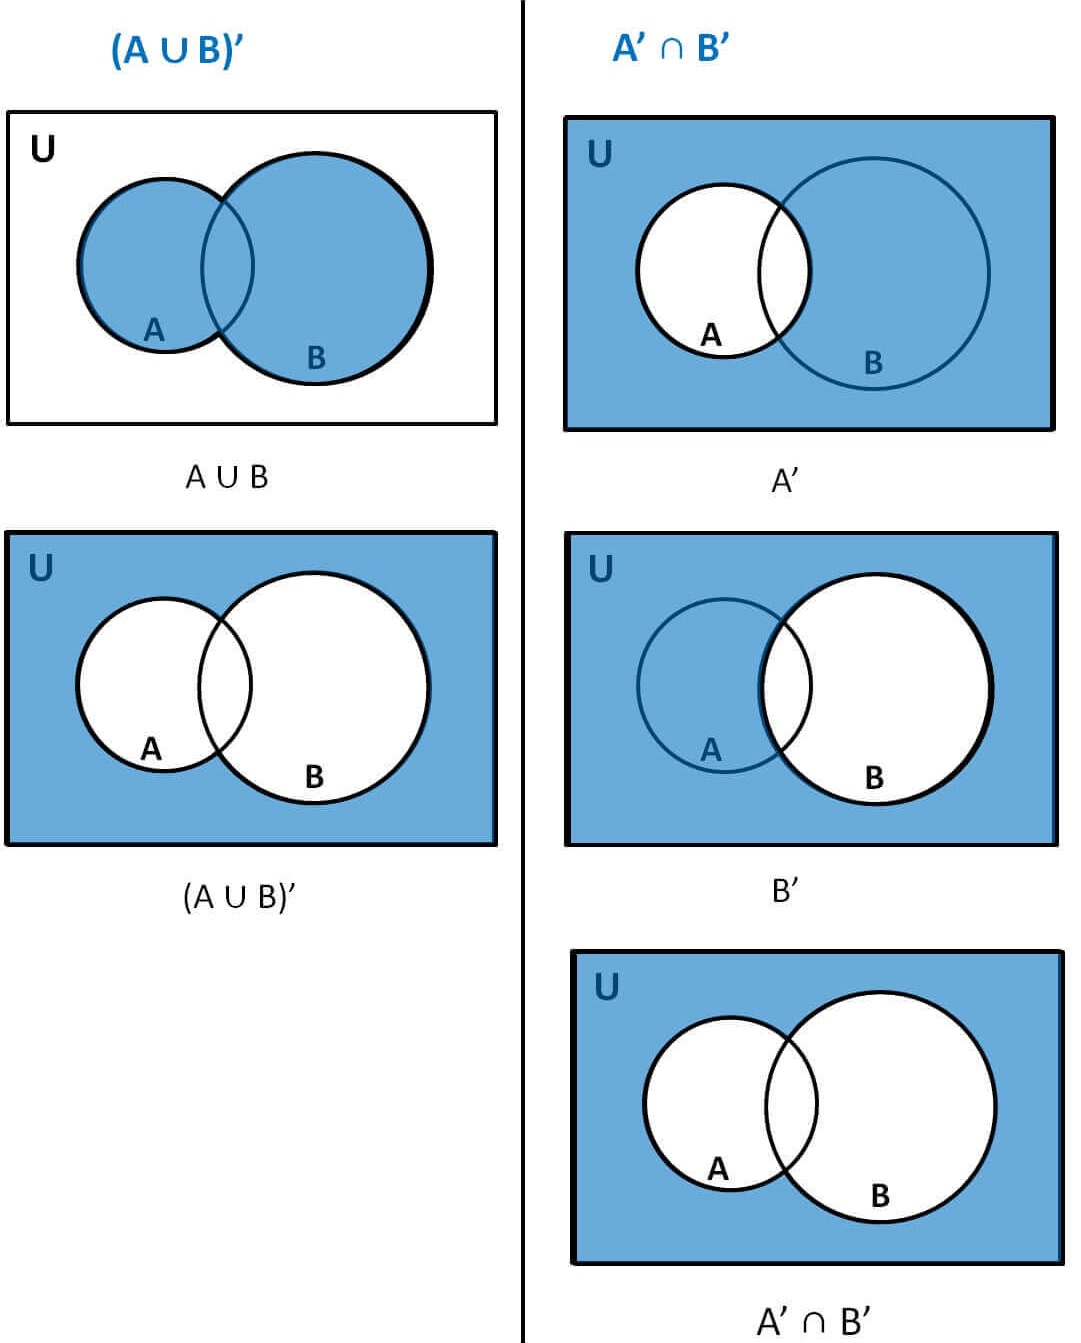
\includegraphics[scale=0.38]{Insiemi/venn-diagram3.jpg}
\end{center}
\framebox{La dimostrazione di 1.2 è molto simile ed è lasciata al lettore} \\
Dimostrazione di (1.2) sotto forma di diagrammi di Venn:
\begin{center}
    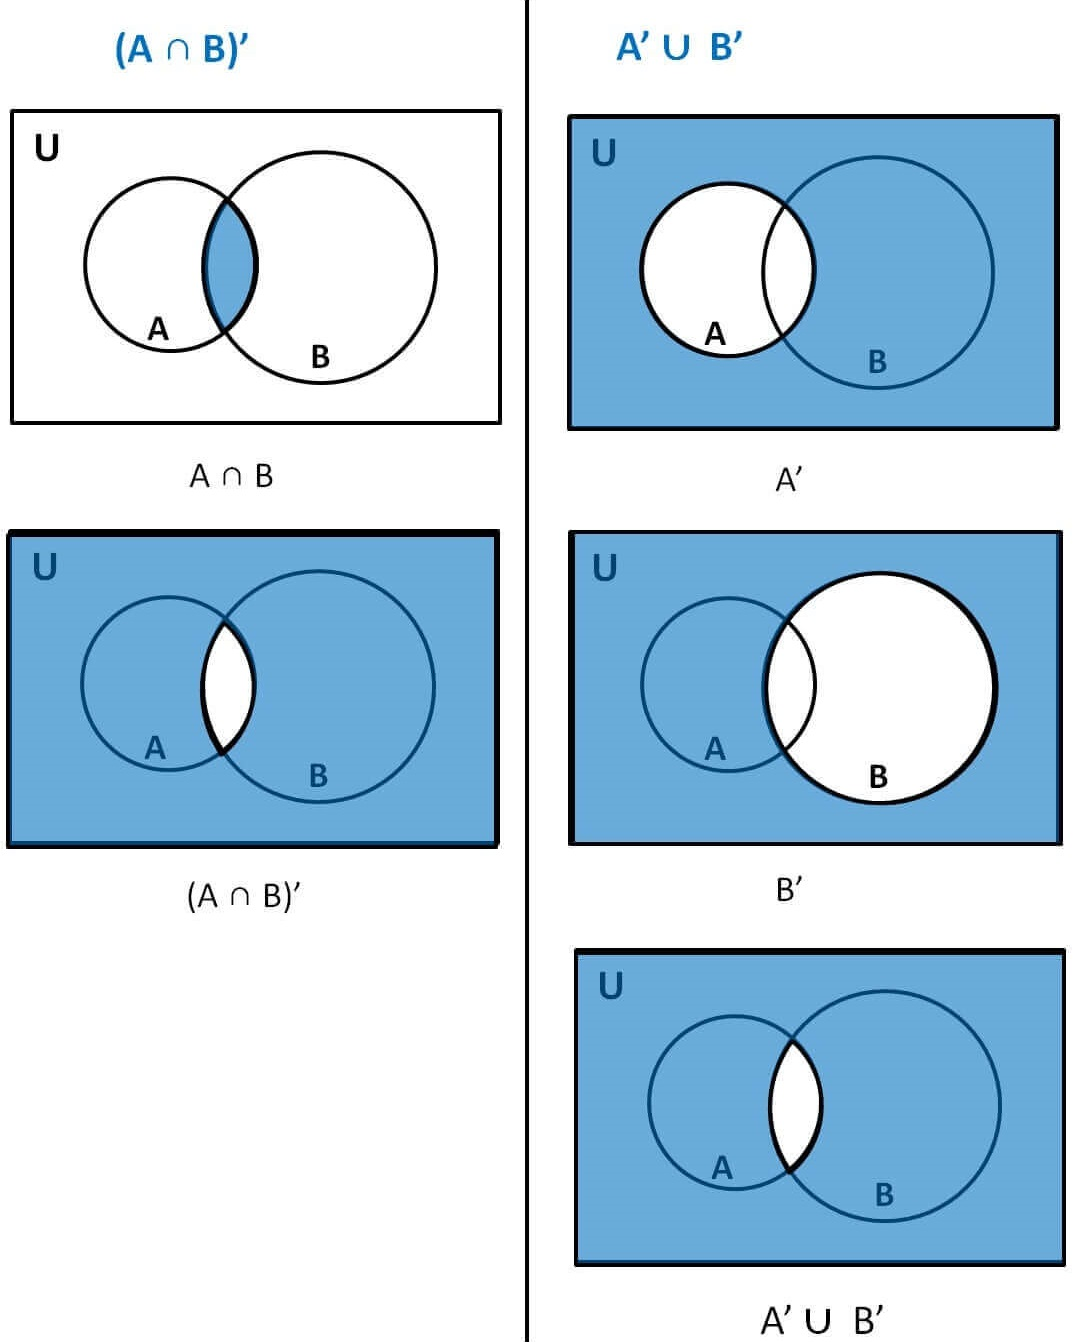
\includegraphics[scale=0.48]{Insiemi/venn-diagram4.jpg}
\end{center}
